\subsection*{Solution 9}

\begin{itemize}
\item[(a)]

\begin{itemize}
\item[(i)]

Let $z=x+iy$, then
\begin{eqnarray*}
f(x+iy)	&=& (x+iy)(3+\overline{x+iy}) + \RE (x+iy) \\
	&=& 3(x+iy) + x^2 + y^2 + x \\
	&=& x^2+y^2+4x + i3y \\
	&=& u(x,y) + iv(x,y)
\end{eqnarray*}
where, $u(x,y) = x^2+y^2+4x$ and $v(x,y) = 3y$.

\item[(ii)]

The function $f$ is defined on $\Complex$. For $u$ and $v$, we have
\[
\begin{array}{ll}
\frac{\partial u}{\partial x} = 2x+4
	& \frac{\partial v}{\partial x} = 0 \\
\\
\frac{\partial u}{\partial y} = 2y
	& \frac{\partial v}{\partial y} = 3
\end{array}
\]
The Cauchy-Riemann equations for the above partial derivatives hold when
$x=-\frac{1}{2}$ and $y=0$.\hbm{A4}{2.1}

Now, $\alpha=\left(-\frac{1}{2},0\right)$, as $f$ is defined on $\Complex$ and the
partial derivatives for $u$ and $v$:
\begin{enumerate}
\item exist on $\Complex$
\item are continuous at $\alpha$
\item satisfy the Cauchy-Riemann equations at $\alpha$
\end{enumerate}
then, by the Cauchy-Riemann Converse Theorem,\hbm{A4}{2.3} $f$ is
differentiable at $\alpha$.

Since $f$ is only differentiable at $\alpha$, then there is no region
where $f$ is analytic and contains $\alpha$, hence $f$ is not analytic
at $\left(-\frac{1}{2},0\right)$.\hbm{A4}{1.3}

\item[(iii)]

From the Cauchy-Riemann Converse Theorem:\hbm{A4}{2.3}
\begin{eqnarray*}
f'\left(-\frac{1}{2}\right)
	&=& \frac{\partial u}{\partial x}\left(-\frac{1}{2},0\right)
		+ i\frac{\partial v}{\partial x}\left(-\frac{1}{2},0\right) \\
	&=& 2\left(-\frac{1}{2}\right) + 4 + i0 \\
	&=& 3
\end{eqnarray*}

\end{itemize}

\item[(b)]

\begin{itemize}
\item[(i)]

Since $g$ is analytic on $\Complex-\{0\}$, with $g'(z) = 1-\frac{i}{z^2}$,
and, since $g'(1)=1-i\ne0$, then $g$ is conformal at $1$.\hbm{A4}{4.6}

\item[(ii)]

With $g(1)=1+i$, $|g'(1)|=|1-i|=\sqrt{2}$ and
$\Arg(g'(1))=-\frac{\pi}{4}$,
the effect of $g$ on a small disc centred at $1$ is to move it to $1+i$,
scale it by $\sqrt{2}$ and rotate it by $\frac{\pi}{4}$ clockwise.\hbm{A4}{1.11}

\item[(iii)]

Since, $\gamma_1(0) = e^{i0} = 1$ and $\gamma_2(1) = (1-1)i+1 = 1$,
then $\gamma_1$ and $\gamma_2$ meet at $t=0$ and $t=1$ respectively.

Let $\theta$ be the angle from $\Gamma_1$ to $\Gamma_2$ at $1$,
then\footnote{From FY's copy of the handbook!}
\hbm{A4}{1.12}
\[
\theta	= \Arg \left( \frac{ \gamma_2'(1) }{ \gamma_1'(0) } \right)
	= \Arg \left( \frac{ ie^{i0} }{ 1+i } \right)
	= \Arg \left( \frac{1}{2} + \frac{i}{2} \right)
	= \frac{\pi}{4}
\]
Hence, at the point of intersection, the angle from $\Gamma_1$ to
$\Gamma_2$ is $\frac{\pi}{4}$.

\item[(iv)]

The paths are shown below:


%
%	Sketches for Q9(b)(iv)
%
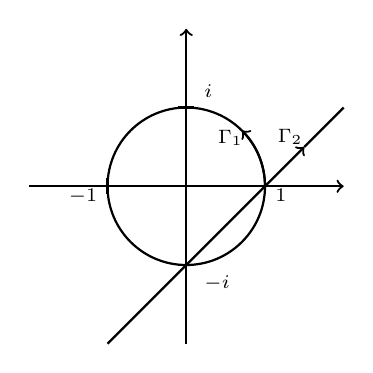
\begin{tikzpicture}
	% grid for draft only
	%%\draw [help lines] (-2,-2) grid (2,2);
	% the X-axis
	\draw[->,thick] (-2,0)--(2,0);
	\draw[thick] (-1,-0.1) -- (-1,0.1) node[below left] {\scriptsize $-1$};
	\draw[thick] (1,-0.1) -- (1,0.1) node[below right] {\scriptsize $1$};
	% the Y-axis
	\draw[->,thick] (0,-2)--(0,2);
	\draw[thick] (-0.1,-1) -- (0.1,-1) node[below right] {\scriptsize $-i$};
	\draw[thick] (-0.1,1) -- (0.1,1) node[above right] {\scriptsize $i$};
	% \Gamma_1
	\draw[thick] (0,0) circle (1);
	\draw[->,thick] (1,0) arc (0:45:1) node[below left=-4pt] {\scriptsize $\Gamma_1$};
	% \Gamma_2
	\draw[->,thick] (-1,-2) -- (1.5,0.5) node[above left=-3pt] {\scriptsize $\Gamma_2$};
	\draw[thick] (1.5,0.5) -- (2,1);
\end{tikzpicture}



\item[(v)]

The directions of $g(\Gamma_1)$ and $g(\Gamma_2)$ are shown below:


%
%	Sketches for Q9(b)(v)
%
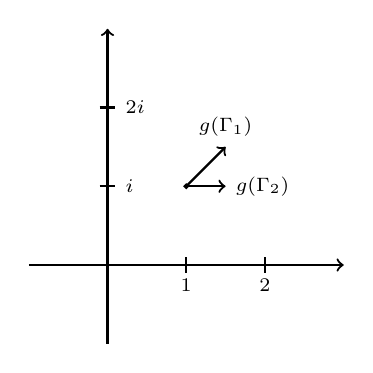
\begin{tikzpicture}
	% grid for draft only
	%%\draw [help lines] (-1,-1) grid (3,3);
	% the X-axis
	\draw[->,thick] (-1,0)--(3,0);
	\draw[thick] (1,-0.1) -- (1,0.1) node[below=4pt] {\scriptsize $1$};
	\draw[thick] (2,-0.1) -- (2,0.1) node[below=4pt] {\scriptsize $2$};
	% the Y-axis
	\draw[->,thick] (0,-1)--(0,3);
	\draw[thick] (-0.1,1) -- (0.1,1) node[right] {\scriptsize $i$};
	\draw[thick] (-0.1,2) -- (0.1,2) node[right] {\scriptsize $2i$};
	% little dot at g(1)
	\draw[thick] (1,1) circle(0.02);
	% g(\Gamma_1)
	\draw[->,thick] (1,1) -- (1.5,1.5) node[above] {\scriptsize $g(\Gamma_1)$};
	% g(\Gamma_2)
	\draw[->,thick] (1,1) -- (1.5,1) node[right] {\scriptsize $g(\Gamma_2)$};
\end{tikzpicture}



\item[(vi)][DC,FY]

The image of the unit circle, $\Gamma(t)=e^{it}$ for $t\in[0,2\pi]$,
under $g$ is as follows:\hbm{A2}{2.5}
\begin{eqnarray*}
g(\Gamma(t))
	&=& g(e^{it}) \\
	&=& e^{it}+ie^{-it} \\
	&=& \cos(t) + i\sin(t) +i(\cos(-t)+i\sin(-t)) \\
	&=& \cos(t)+i\sin(t)+i\cos(t)-i^2\sin(t) \\
	&=& (\cos(t)+\sin(t))(1+i)
\end{eqnarray*}

\end{itemize}

\end{itemize}

